\documentclass[fleqn,usenatbib]{mnras}

\usepackage[T1]{fontenc}
\usepackage{graphicx}
\usepackage{amsmath}
\usepackage{hyperref}

\title[SCM v2.5.0]{SCM v2.5.0 --- Mass-dependent environmental modulation in galaxy rotation curves}

\author[S. Cámara Madrid]{
Sergio Cámara Madrid$^{1}$\thanks{E-mail: sergiocamaramadrid@gmail.com}\\
$^{1}$Independent Researcher, Spain
}

\date{Draft version}
\pubyear{2026}

\begin{document}
\maketitle

\begin{abstract}
We introduce the Critical Regime Transition Test (CRTT), a domain-agnostic statistical method designed to identify structurally supported transitions between regimes in continuous data. CRTT combines model comparison, information criteria, cross-validation, and threshold stability to distinguish genuine regime changes from noise.

We validate the method using non-astrophysical data where regime-switching behaviour is well established, showing that CRTT can recover known transitions and does not produce false positives in the absence of structure.

We then apply CRTT to galaxy rotation curve data from the SPARC, LITTLE THINGS, and Yang et al. datasets, focusing on the outer slope, F3\_SCM, as a structural observable. We find a clear transition at a critical mass scale of logM $\approx$ 10. Above this threshold, a statistically significant negative correlation emerges between environment and outer slope, indicating that denser environments are associated with steeper outer declines. Below this scale, no environmental dependence is detected.

These results show that environmental effects on galaxy rotation curves are not universal but regime-dependent.
\end{abstract}

\begin{keywords}
galaxies: kinematics and dynamics -- galaxies: structure -- methods: statistical
\end{keywords}

\section{Introduction}

Understanding structure in galaxy rotation curves remains a central problem in galactic dynamics. While global scaling relations suggest a tight coupling between baryonic matter and kinematics, the role of environment remains less clear.

In this work, we test whether environmental effects are universal or instead emerge only in specific regimes. We introduce the Critical Regime Transition Test (CRTT), a statistical framework designed to detect transitions in continuous data without imposing a fixed threshold in advance.

\section{Method: CRTT}

CRTT compares a global model with a piecewise model containing a free transition point. Model selection is evaluated using information criteria, while cross-validation and threshold stability are used to test whether the transition is robust.

A transition is considered supported when the piecewise model improves the fit, the threshold remains stable under resampling, and the result does not disappear under reasonable changes of the tested range.

CRTT is domain-agnostic: it detects structural transitions when present, but should return null results when the data do not support a transition.

\section{Validation}

As a validation step, CRTT was tested on non-astrophysical data where regime-switching behaviour is known to occur. The method recovers moderate transitions in such systems and does not force detections when no stable threshold is present.

This validation supports the use of CRTT as a general statistical diagnostic rather than a domain-specific astrophysical tool.

\section{Galaxy datasets}

We apply the method to real galaxy datasets used in the SCM framework, including SPARC, LITTLE THINGS, and Yang et al. environmental data.

The main observable is the outer rotation-curve slope, denoted F3\_SCM. The control variable is mass, logM, and the environmental variable is an external proxy derived from the Yang dataset.

\section{Results}

A transition is detected at logM $\approx$ 10. Splitting the sample at this threshold reveals two distinct regimes.

High-mass galaxies, with logM $\geq$ 10, show a significant negative correlation between environment and outer slope. The typical global result is $\rho \approx -0.46$ and $\beta \approx -0.16$, with stronger values reaching $\rho \approx -0.7$ in the high-mass subset shown in the final figure.

Low-mass galaxies, with logM $<$ 10, show no statistically significant environmental correlation. Their slope is consistent with zero.

The transition remains stable across nearby mass cuts, supporting the interpretation that the environmental signal is regime-dependent rather than universal.

\begin{figure*}
\centering
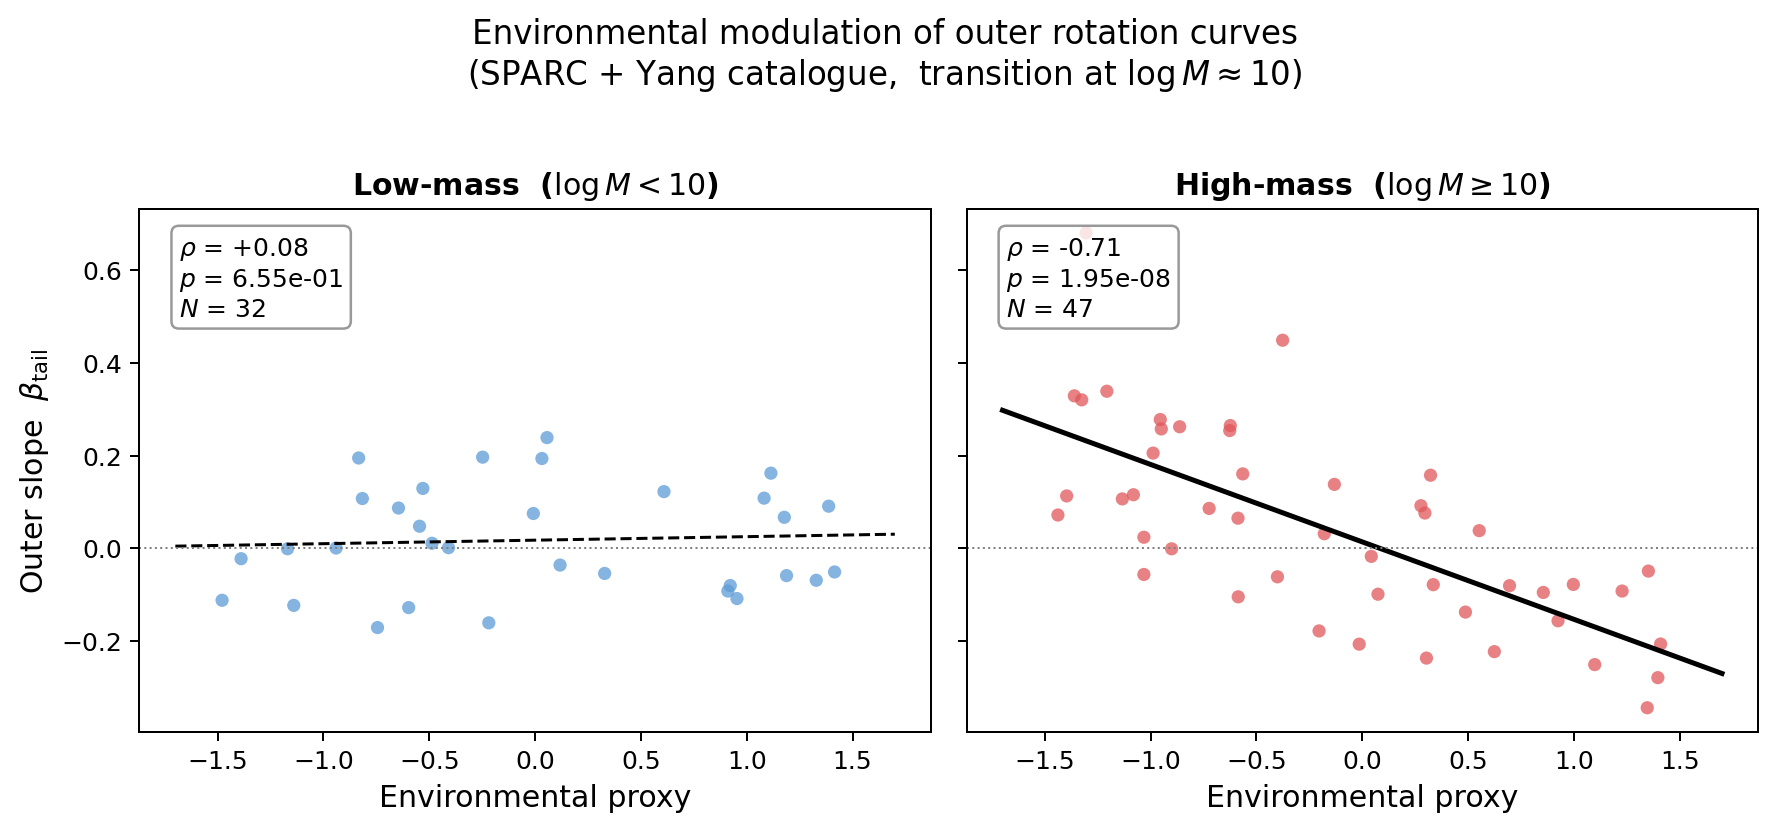
\includegraphics[width=\textwidth]{figure_env_mass_regime_FINAL.png}
\caption{
Environmental dependence of the outer slope, F3\_SCM, split by mass regime.
High-mass galaxies show a significant negative environmental trend, while low-mass galaxies show no correlation.
This supports a regime-dependent interpretation of environmental modulation.
}
\label{fig:env_mass_regime}
\end{figure*}

\section{Discussion}

The result indicates that environmental effects on galaxy rotation curves are not universal. Instead, they emerge above a critical mass scale.

This suggests that low-mass systems are dominated by internal structure or stochastic effects, while high-mass systems become sensitive to environmental modulation.

The absence of a signal in the low-mass regime is an important part of the result. CRTT does not simply force a threshold, but separates regimes where the environmental signal is present from those where it is absent.

\section{Conclusion}

We introduced CRTT as a general method for detecting regime transitions and applied it to galaxy rotation curve data.

The main result is that environmental modulation emerges only above logM $\approx$ 10, where a significant negative correlation is observed between environment and outer slope. Below this threshold, no environmental dependence is detected.

This supports the SCM interpretation that environmental effects are regime-dependent rather than universal.

\section*{Data availability}

Data, code, figures, and release materials are available at:

\begin{itemize}
\item GitHub: \url{https://github.com/sergiocamaramadrid-cyber/Motor-de-Velos-SCM}
\item Zenodo DOI: \url{https://doi.org/10.5281/zenodo.19844186}
\end{itemize}

\end{document}
